\documentclass[twocolumn]{ctexart}
\usepackage{ctex}
\usepackage{amsmath}

%首行缩进两字符 利用\indent \noindent进行控制
\usepackage{indentfirst}
\setlength{\parindent}{2em}

%算法包
\usepackage{caption}
\usepackage{algorithm}
\usepackage{algorithmic}

%页边距包
\usepackage{geometry}
\geometry {left=2.0cm ,right=2.0cm,top=2.5cm,bottom=2.5cm}

%枚举
\usepackage{enumerate}

%算法input output
\renewcommand{\algorithmicrequire}{\textbf{Input:}} % Use Input in the format of Algorithm
\renewcommand{\algorithmicensure}{\textbf{Output:}} % Use Output in the format of Algorithm

%数学符号
\usepackage{amssymb}
\usepackage{wasysym}
%图片
\usepackage{graphicx}

%表格
\usepackage{booktabs}
\usepackage{multirow}

%Tikz画图
\usepackage{tikz}
\usetikzlibrary{arrows,graphs} %指明是图库
\usetikzlibrary{positioning,automata}

%\usegdlibrary
\begin {document}
	\title{Problem Set 5 Answer Sheet}
	\author{\textbf{151220131谢旻晖}}
	\date{}
	\maketitle

\section*{Problem 6.1}
\indent $n-2$

\section*{Problem 6.2}
\noindent 1.\\
\indent 第一个点是我们手动设定的,无需比较。\\
\indent
从第二个点开始,每次$getMin$将第$i$个节点加入$tree$,要对所有$fringe$的点中比较以得最小权者($n-i$次cmp),同时需要对所有其他的$fringe$点进行$updateFringe$($n-i$次cmp)。\\
\[
	\sum_{i=2}^{n}n-i+n-i=(n-1)(n-2)
\]
\\
\noindent 2.\\
\indent $n-1$

\section*{Problem 6.5}
\noindent 1.\\
\indent 将图所有边权取负,求新图的MST,再将所有边权恢复,MST即为最大权重生成树。\\
\noindent 2.\\
\indent 求最大权重生成树的补图,其中所有的边形成的集合为最小的反馈边集。

\section*{Problem 6.6}
\indent 是不可能的。下面证明:最短路径树与任何最小生成树都至少共用一条边。\\
\indent 证明:考虑从$s$点开始,我们使用$Prim$算法构造MST的过程,第一步,我们从所有与$s$相连的边中选出权最小的那条边(设为$s\rightarrow v$),此时我们就保证了$s$到$v$的最短路径是$s\rightarrow v$,换而言之,$s\rightarrow v$一定既在MST中,又在SSSPT中。证毕。

\section*{Problem 6.7}
\noindent\textbf{case a:}仍然不变\\
\textbf{case b:}把修改的边加入原生成树,在生成的环中去掉权值最大的边(破圈)\\
\textbf{case c:}仍然不变\\
\textbf{case d:}将修改的边删除,原生成树形成两个连通分量,可以用SCC算法识别出两个连通分量,接着遍历所有的边,找到其中权值最小的且连接两个连通分量的边,加入。\\


\section*{Problem 6.8}
\indent 令$\varPhi=V-U$,$\varPsi=\{(x,y)|x,y\in\varPhi \wedge (x,y)\in E\}$,首先考虑图$G'=(\varPhi,\varPsi)$的MST,如果$G'$都不连通,则最轻生成树显然不存在,如果连通,我们求出$G'$的最小生成树$T$。\\
\indent 接着考虑边集$\Gamma=\{(x,y)|x\in\varPhi \wedge y\in U \wedge (x,y)\in E \}$
,不断选$\Gamma$中权值最小的边加入$T$,以将$U$中的结点连接至$T$,已连接过的结点不再重复连接。直到将$U$中的结点全部连接完毕,$T$为最轻生成树。若$U$中有点与$T$不连通,则不存在最轻生成树。

\section*{Problem 6.9}
\indent $Krystal$改进版本:设G的边集为E,首先将S中的所有边选入,然后在E-S中不断选不与已选边构成环且权值最小的边,直到总共选满$|G.V|-1$条边。

\section*{Problem 6.11}
\noindent 命题正确。\\
\indent $\Rightarrow$\\
\indent 采用反证法,如果$T$是$G$的MST,但$T$不是$G'$的MST。那么$G'$一定存在一个权值比$T$小的最小生成树$T'$。根据平方关系,$T'$在$G$中的权也小于$T$,与$T$是$G$的MST矛盾,假设不成立。所以$T$是$G$的最小生成树,那$T$一定也是$G'$的最小生成树。\\

\indent $\Leftarrow$\\
\indent 同理。

\section*{Problem 6.12}
\noindent1.\\
\indent 采用反证法证明,若存在两个最小生成树$T_1$和$T_2$,我们找出权值最小的$T_1$和$T_2$中不同的边$e$,不失一般性,不妨设他在$T_1$但不在$T_2$中。\\
\indent
根据MST Property,在$T_2$中加入$e$,则构成圈且有$e$为圈中权值最大的边,若圈中其他非$e$的边都是$T_1$中的边,则这些边和$e$就会在$T_1$构成圈,与$T_1$为MST矛盾,所以\textbf{必定有}某条边$x$在$T_2$但不在$T_1$中。\\
\indent 由MST Property,$x$的权<$e$的权,这与$e$是\textbf{权值最小}的的$T_1$和$T_2$中不同的边矛盾。所以假设不成立。\\

\noindent 2.\\
\begin{center}
	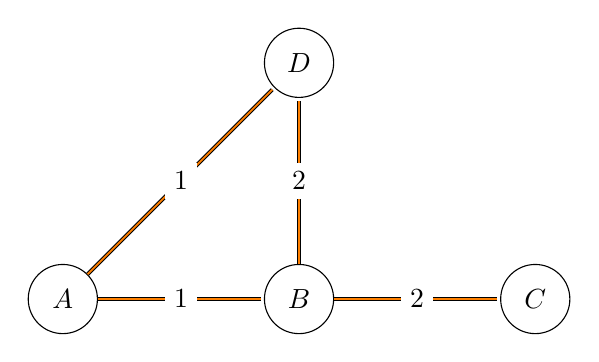
\begin{tikzpicture}[>=stealth',shorten >=1pt,node distance=3cm,on grid,initial/.style    ={}]
	\node[state]          (A)                        {$A$};
	\node[state]          (B) [right =of A]    {$B$};
	\node[state]          (C) [right =of B]    {$C$};
	\node[state]          (D) [above =of B]    {$D$};
	\tikzset{every node/.style={fill=white}} 
	\tikzset{mystyle/.style={-,double=orange}}   
	\path
	(A)     edge [mystyle]   node   {$1$} (B)
	(A)     edge [mystyle]   node   {$1$} (D) 
	(B)     edge [mystyle]   node   {$2$} (D)
	(B)     edge [mystyle]   node   {$2$} (C);
	\end{tikzpicture}
\end{center}


\noindent 3.\\
\indent 给出图显然具有唯一的MST,但他两个条件均不满足。\\
\begin{center}
	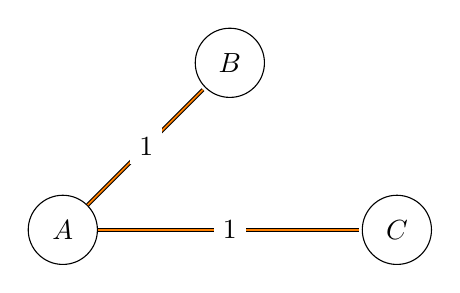
\begin{tikzpicture}[>=stealth',shorten >=1pt,node distance=3cm,on grid,initial/.style    ={}]
	\node[state]          (A)                        {$A$};
	\node[state]          (B) [above right =of A]    {$B$};
	\node[state]          (C) [below right =of B]    {$C$};
	\tikzset{every node/.style={fill=white}} 
	\tikzset{mystyle/.style={-,double=orange}}   
	\path
	(A)     edge [mystyle]   node   {$1$} (B)
	(A)     edge [mystyle]   node   {$1$} (C);
	\end{tikzpicture}
\end{center}

\noindent 4.\\
\indent 可以将MST Property拓宽为Unique MST Property.他的定义为:向ST中加入任意一条边$e$,在形成的圈中,$e$的权最大且没有和他一样大的边。可以很容易的证明一棵树具有Unique MST Property性质,那就具有题意的唯一性。\\
\indent 为此,给出算法如下:在构造出MST之后,遍历$E$-MST,不断向MST中加入边,如果在形成的圈中它的权最大且没有和它一样大的,那么OK,否则则不唯一。

%\section*{Problem 6.13}
%\noindent1.\\
%\indent 易证,有用边一定是割边,肯定在MST中。\\
%
%\noindent2.\\
%\indent 如果有危险边,
%
%\noindent3.\\

\section*{Problem 6.14}
\indent 容易举出一个反例\\
\begin{center}
	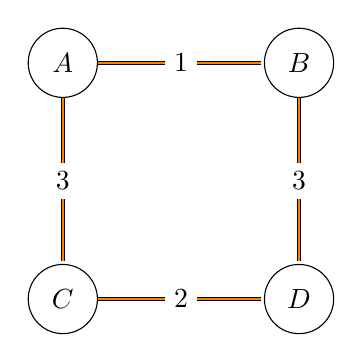
\begin{tikzpicture}[>=stealth',shorten >=1pt,node distance=3cm,on grid,initial/.style    ={}]
	\node[state]          (A)                        {$A$};
	\node[state]          (B) [right =of A]    {$B$};
	\node[state]          (C) [below =of A]    {$C$};
	\node[state]          (D) [below =of B]    {$D$};
	\tikzset{every node/.style={fill=white}} 
	\tikzset{mystyle/.style={-,double=orange}}   
	\path
	(A)     edge [mystyle]   node   {$1$} (B)
	(A)     edge [mystyle]   node   {$3$} (C) 
	(C)     edge [mystyle]   node   {$2$} (D)
	(B)     edge [mystyle]   node   {$3$} (D);
	
%	\draw [dashed] (1.5,1.3)--(1.5,-3);
	
	\end{tikzpicture}
\end{center}

\indent 如图所示,令$V_1=\{A,C\}$,$V_2=\{B,D\}$,利用题意中的分治算法求出的MST为\{AB,AC,BD\},权为7,而实际上的最小生成树为\{AB,CD,AC\}或\{AB,CD,BD\},权为6。

\section*{Problem 6.15}
\indent 首先,如果一个生成树是第二小的生成树,那么他一定与某棵最小生成树仅有一边之差。然后,先用$Kruskals$算法求出原图的MST,接着我们尝试删去MST中的每条边,在此基础上再次运行$Kruskals$算法构建生成树(注意不能用刚刚删去的边),计算此树与MST的权差,找到其中权差最小但\textbf{非0}(避免找到MST)的ST,即为次小生成树。\\


\section*{Problem 6.16}
在此图上运行$Dijkstra$算法,源点为S,会错误地得到S->B的最短路径为2的结论。
\begin{center}
	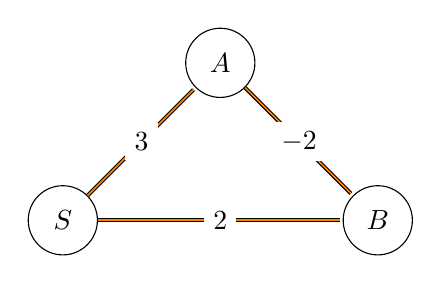
\begin{tikzpicture}[>=stealth',shorten >=1pt,node distance=3cm,on grid,initial/.style    ={}]
	\tikzset{every node/.style={circle}}
	\node[state] (A) at (0,0)        {$S$};
	\node[state] (B) at (2,2)        {$A$};
	\node[state] (C) at (4,0)        {$B$};
	\tikzset{every node/.style={fill=white}} 
	\tikzset{mystyle/.style={-,double=orange}}   
	\path
	(A)     edge [mystyle]   node   {$3$} (B)
	(A)     edge [mystyle]   node   {$2$} (C) 
	(B)     edge [mystyle]   node   {$-2$} (C);
	
	\end{tikzpicture}
\end{center}
\indent$Dijkstra$由于是贪心的,每次都找一个距源点最近的点(dmin),然后将该距离定为这个点到源点的最短路径(d[i]<--dmin);但如果存在负权边,那就有可能先通过并不是距源点最近的一个次优点,再通过这个负权边生成的路径之和更小。

\section*{Problem 6.17}
\indent 给定源点为S,在下图中生成的最短路径树为\{SA,SB\},但MST为\{SB,BA\}。
\begin{center}
	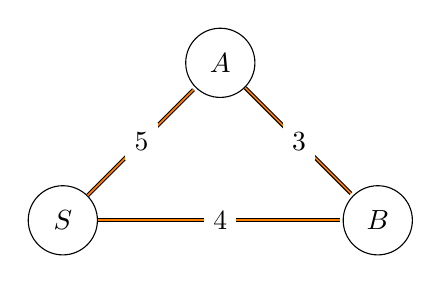
\begin{tikzpicture}[>=stealth',shorten >=1pt,node distance=3cm,on grid,initial/.style    ={}]
	\tikzset{every node/.style={circle}}
	\node[state] (A) at (0,0)        {$S$};
	\node[state] (B) at (2,2)        {$A$};
	\node[state] (C) at (4,0)        {$B$};
	\tikzset{every node/.style={fill=white}} 
	\tikzset{mystyle/.style={-,double=orange}}   
	\path
	(A)     edge [mystyle]   node   {$5$} (B)
	(A)     edge [mystyle]   node   {$4$} (C) 
	(B)     edge [mystyle]   node   {$3$} (C);
	
	\end{tikzpicture}
\end{center}

\section*{Problem 6.18}
\begin{algorithm}[htbp]
	\caption{UNIQUE\_SSSP}
	\label{uniquesssp}
	\begin{algorithmic}[1]
		\REQUIRE{Graph}
		\ENSURE	{U[0...|V|-1]}
		\STATE status[0...n-1],fringeWgt[0...n-1]
		\STATE Priority Queue pq=create(n,status,fringeWgt)
		\STATE pq.insert(s)
		\STATE U[0...|V|-1]=FALSE
		\WHILE {!pq.isEmpty}
		\STATE v=pq.top()
		\STATE pq.pop()
		\STATE //updateFringe
		\STATE myDist=fringeWgt[v]
		\FOR{\textbf{each} vertex w in v.Adj}
		\STATE newDist=myDist+weight($v->w$)
		\IF{status[w]==unseen}
		\STATE pq.insert(w)
		\ELSIF {status[w]==fringe}
		\IF{newDist<getPriority(pq,w)}
		\STATE decreaseKey(pq,w,v,newDist)
		\ENDIF
		\ELSE	
		\IF{newDist==myDist}
		\STATE U[w]=TRUE
		\ENDIF
		\ENDIF
		\ENDFOR
		\ENDWHILE
		U[s]=TRUE
	\end{algorithmic}
\end{algorithm}

\indent 对$Dijkstra$算法的松弛部分稍作改动即可,在松弛部分,若$fringe结点$更新后的权与某个$tree$/$finished$结点v的distance相同,则v的最短路径不唯一,$U[v]=TRUE$。\\
\indent 在Sara Baase教材的算法上作改动。其中Priority Queue的实现,status的定义,decreaseKey、insert、pop、top等函数的实现均与课本相同。\\
\indent 算法伪代码见\textbf{Algorithm \ref{uniquesssp}}. 






\section*{Problem 6.19}
\noindent 1.\\
\indent 没有变。证明:设原来的最小生成树为$T$,加了权之后的生成树为$T'$,下面证明$T'$仍然具有MST Property:向$T'$中加入任意的一条边$e'$,形成一个圈,显然$e'$是圈中权值最大的边,因为在$T$中加入与$e'$对应的$e$形成的圈中$e$是权值最大的边,所有边权值加一之后仍然是这样。\\
\indent 因为$T'$具有MST Property,它仍然是MST。\\

\noindent 2.\\
\indent 会变化。\\
\begin{center}

	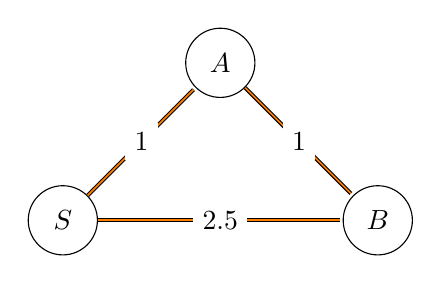
\begin{tikzpicture}[>=stealth',shorten >=1pt,node distance=3cm,on grid,initial/.style    ={}]
	\tikzset{every node/.style={circle}}
	\node[state] (A) at (0,0)        {$S$};
	\node[state] (B) at (2,2)        {$A$};
	\node[state] (C) at (4,0)        {$B$};
	\tikzset{every node/.style={fill=white}} 
	\tikzset{mystyle/.style={-,double=orange}}   
	\path
	(A)     edge [mystyle]   node   {$1$} (B)
	(A)     edge [mystyle]   node   {$2.5$} (C) 
	(B)     edge [mystyle]   node   {$1$} (C);
	
	\end{tikzpicture}

	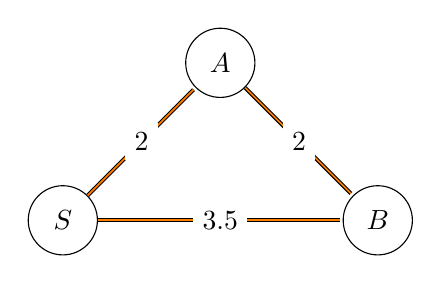
\begin{tikzpicture}[>=stealth',shorten >=1pt,node distance=3cm,on grid,initial/.style    ={}]
	\tikzset{every node/.style={circle}}
	\node[state] (A) at (0,0)        {$S$};
	\node[state] (B) at (2,2)        {$A$};
	\node[state] (C) at (4,0)        {$B$};
	\tikzset{every node/.style={fill=white}} 
	\tikzset{mystyle/.style={-,double=orange}}   
	\path
	(A)     edge [mystyle]   node   {$2$} (B)
	(A)     edge [mystyle]   node   {$3.5$} (C) 
	(B)     edge [mystyle]   node   {$2$} (C);
	\end{tikzpicture}
\end{center}
\indent 原来$S\leadsto B$的最短路径为$S\to A\to B$,在所有边权值加一之后,$S\leadsto B$的最短路径为$S\to B$.\\

\section*{Problem 6.20}
\begin{algorithm}[htbp]
	\caption{Extended\_SSSP}
	\label{ExtendedSSSP}
	\begin{algorithmic}[1]
		\REQUIRE{Graph}
		\ENSURE	{U[0...|V|-1]}
		\STATE status[0...n-1],fringeWgt[0...n-1]
		\STATE Priority Queue pq=create(n,status,fringeWgt)
		\STATE pq.insert(s)
		\STATE fringeWgt[s]=$c_s$ //初始化自己的权值为$c_s$
		\STATE U[0...|V|-1]=FALSE
		\WHILE {!pq.isEmpty}
		\STATE v=pq.top()
		\STATE pq.pop()
		\STATE //updateFringe
		\STATE myDist=fringeWgt[v]
		\FOR{\textbf{each} vertex w in v.Adj}
		\STATE newDist=myDist+weight($v->w$)+weight(w)//不仅加边的权,还加点的权
		\IF{status[w]==unseen}
		\STATE pq.insert(w)
		\ELSIF {status[w]==fringe}
		\IF{newDist<getPriority(pq,w)}
		\STATE decreaseKey(pq,w,v,newDist)
		\ENDIF
		\ELSE	
		\IF{newDist==myDist}
		\STATE U[w]=TRUE
		\ENDIF
		\ENDIF
		\ENDFOR
		\ENDWHILE
		U[s]=TRUE
	\end{algorithmic}
\end{algorithm}

\indent 在$Dijkstra$算法的基础上稍作改动,初始化时令Cost[s]=$c_s$,将框架中的"$newDist = myDist+weightEdge$"改为"$newDist = myDist+weightEdge+weightVertex$",其余不变。\\
\indent 
算法伪代码见\textbf{Algorithm \ref{ExtendedSSSP}}。\\


\section*{Problem 6.21}
\indent 适用。\\
\indent 首先原图中我们认为没有负权圈,否则就可以一直转,无意义。\\
\indent 为什么普通的带负权的边$Dijkstra$会失败呢?由于是贪心的,每次都找一个距源点最近的点(dmin),然后将该距离定为这个点到源点的最短路径(d[i]<--dmin);但如果存在负权边,那就有可能先通过并不是距源点最近的一个次优点,再通过这个负权边生成的路径之和更小。\\
\indent 即$s\leadsto v_i \to v_j$,有可能存在$s\leadsto v_i$ $\underrightarrow{negative}$  $ v_j$,使得$dist(v_j)<dist(v_i)$。\\
\indent 而在所有负权边都从源点发出的条件下,我们没有了$v_i$,也就没有这种问题了。我们无法通过负权边,使得一个已经被添加进最短路径树(换言之,已经固定下来的),找到一个比他更短的path。

\section*{Problem 6.23}
\noindent 1.\\
\indent 设油箱容量为L,在s处进行DFS遍历,遍历的规则是如果边权大于L,就不继续遍历;小于等于L,才继续往深里走。若遍历到了t节点,则存在一条可行路径,否则不存在。\\

\noindent 2.\\
\indent $Dijkstra$算法变形,在s处求单源结点的最短"路径",只是将框架中的"$newDist = myDist+weight$"改为"$newDist = max(myDist,weight)$",其余不变。最后输出$s\leadsto t$的最短"路径"为油箱最小容量。\\

\section*{Problem 6.25}
\begin{algorithm}[htbp]
	\caption{FloydWarshallWithGoPath}
	\label{FloydGo}
	\begin{algorithmic}[1]
		\STATE fill dist[ ][ ] with $\infty$ and GO[ ][ ] with $NUL$
		\FOR{\textbf{each} edge (u,v)}
		\STATE dist[u][v]=w(u,v)  // the weight of the edge (u,v)
		\STATE GO[u][v]=v
		\ENDFOR
		\FOR{k from 1 to |V|}
		\FOR{ i from 1 to |V|}
		\FOR{ j from 1 to |V|}
		\IF{dist[i][j] > dist[i][k] + dist[k][j]}
		\STATE 	dist[i][j]=dist[i][k] + dist[k][j]
		\STATE	GO[i][j]=GO[i][k]
		\ENDIF
		\ENDFOR
		\ENDFOR
		\ENDFOR
	\end{algorithmic}
\end{algorithm}

\noindent 1.算法见\textbf{Algorithm \ref{FloydGo}}\\

\begin{algorithm}[htbp]
	\caption{FloydWarshallWithBackPath}
	\label{FloydBack}
	\begin{algorithmic}[1]
		\STATE fill dist[ ][ ] with $\infty$ and BACK[ ][ ] with $NUL$
		\FOR{\textbf{each} edge (u,v)}
		\STATE dist[u][v]=w(u,v)  // the weight of the edge (u,v)
		\ENDFOR
		\FOR{k from 1 to |V|}
		\FOR{i from 1 to |V|}
		\FOR{j from 1 to |V|}
		\IF{dist[i][j] > dist[i][k] + dist[k][j]}
		\STATE 	dist[i][j]=dist[i][k] + dist[k][j]
		\STATE	BACK[i][j]=BACK[k][j]
		\ENDIF
		\ENDFOR
		\ENDFOR
		\ENDFOR
	\end{algorithmic}
\end{algorithm}

\noindent2.算法见\textbf{Algorithm \ref{FloydBack}}\\


\section*{Problem 6.31}
\indent 利用一个数组income记录这个结点接受到的path的数量,使用BFS,每当上层结点遍历到下一层结点时,下一层结点的income+=上层结点的income值。直到遍历完v为止。\\
\indent 更为具体地,由于无向图只有Tree Edge和Cross Edge。初始化时,初始化所有的income=0,接着从源点进行BFS遍历,若碰到Tree Edge (x,y),则income[y]+=income[x];若碰到Cross Edge,则忽略(因为不是最短路径了)。算法结束后的income[v]即为所求值。 

\end {document}
